% !TEX encoding = UTF-8 Unicode
\documentclass{beamer}

\usepackage{amsmath}
\usepackage{color}
\usepackage{gensymb}
\usepackage{hyperref}
\usepackage{textcomp}
\usepackage{wasysym}

\usepackage{listings}
\usepackage{listings}
\lstset{language=Python,
    basicstyle=\ttfamily\bfseries,
    commentstyle=\color{red}\itshape,
    stringstyle=\color{darkolivegreen},
    showstringspaces=false,
    keywordstyle=\color{blue}\bfseries}

\usetheme{Warsaw}

\newcommand{\btVFill}{\vskip0pt plus 1filll}

\definecolor{darkolivegreen}{rgb}{0.33, 0.42, 0.18}

\title[Daily monitoring of low-frequency earthquake activity]{Daily monitoring of low-frequency earthquake activity}
\author{Ariane Ducellier, Scott Henderson}
\date{Winter 2020 Incubator project}

\begin{document}

	\begin{frame}
		\titlepage
	\end{frame}

	\begin{frame}
		\frametitle{Low-frequency earthquakes (LFEs)}
		\begin{itemize}
			\item Small magnitude (M $\sim$ 1)
			\item Dominant frequency low (1-10 Hz) compared with that of ordinary tiny earthquakes (up to 20 Hz)
			\item Source located on the plate boundary
			\item Grouped into families of events, with all the earthquakes of a given family originating from the same small patch on the plate interface
			\item Recurrence more or less episodic in a bursty manner
		\end{itemize}
	\end{frame}

	\begin{frame}
		\frametitle{What we do now}
		\begin{itemize}
			\item Download seismic data for a given period of time
			\item Analyze data and find time of occurrence of LFEs
			\item Create a catalog of LFEs for a given period of time and publish it
		\end{itemize}
	\end{frame}

	\begin{frame}
		\frametitle{What we aim to do}
		\begin{itemize}
			\item Low-frequency earthquake occur and are recorded by permanent seismic stations every day
			\item On a daily basis:
			\begin{itemize}
				\item Download seismic data from the day before
				\item Analyze data and find low frequency earthquakes
				\item Update the catalog
			\end{itemize}
		\end{itemize}
	\end{frame}

	\begin{frame}[fragile]
		\frametitle{First step: Python package}
		\scriptsize{
		\begin{columns}[c]
			\begin{column}{5cm}
				\begin{block}{catalog}
				\begin{itemize}
					\item	Specific Python scripts for downloading data and finding LFEs
					\item Directory with templates for two LFE families
				\end{itemize}
				\end{block}
				\begin{block}{utils}
				General Python scripts for stacking and cross-correlation
				\end{block}
				\begin{block}{data}
				\begin{itemize}
					\item File with list of LFE families
					\item File with list of seismic stations
					\item Directory with instrument response from seismic stations
				\end{itemize}
				\end{block}
			\end{column}
			\begin{column}{1cm}
				\centering
				\Huge\pointer
			\end{column}
			\begin{column}{5cm}
				\begin{block}{lfelib}
				\begin{itemize}
					\item Specific Python scripts for downloading data and finding LFEs
					\item \verb+utils+ : General Python scripts for stacking and cross-correlation
				\end{itemize}
				\end{block}
				\begin{block}{tests}
				\end{block}
				\begin{block}{examples}
				Templates, instrument responses, list of LFE families and seismic stations
				\end{block}
				\begin{block}{.github/workflows}
				\end{block}
				\begin{itemize}
					\item environment.yml
					\item pyproject.toml
				\end{itemize}
			\end{column}
		\end{columns}
		}
	\end{frame}

	\begin{frame}[fragile]
		\frametitle{Second step: Command line}
		\begin{exampleblock}{}
		\scriptsize{
		\begin{lstlisting}
		> python
		>>>  get_all_responses('stations_permanent.txt')
		>>>  find_LFEs('families_permanent.txt', \
		    'stations_permanent.txt', 'templates', \
		    (2020, 3, 7, 0, 0, 0), (2020, 3, 8, 0, 0, 0), 10.0, \
		    60.0, (1.5, 9.0), 1.0, 0.05, 10, 10.0, 'MAD', 8.0)
		\end{lstlisting}
		}
		\end{exampleblock}

		\centering
		\Huge{
		$\Downarrow$
		}

		\begin{exampleblock}{}
		\scriptsize{
		\begin{verbatim}
		getresp -s stations_permanent.txt

		lfeall -ff families_permanent.txt -s stations_permanent.txt 
		-t templates -t0 $year1 $month1 $day1 0 0 0
		-tf $year2 $month2 $day2 0 0 0 -td 10.0 -d 60.0
		-f 1.5 9.0 -f0 1.0 -dt 0.05 -n 10 -w 10.0 -tr MAD -tv 8.0
		\end{verbatim}
		}
		\end{exampleblock}
	\end{frame}

	\begin{frame}
		\frametitle{Third step: GitHub workflow}
		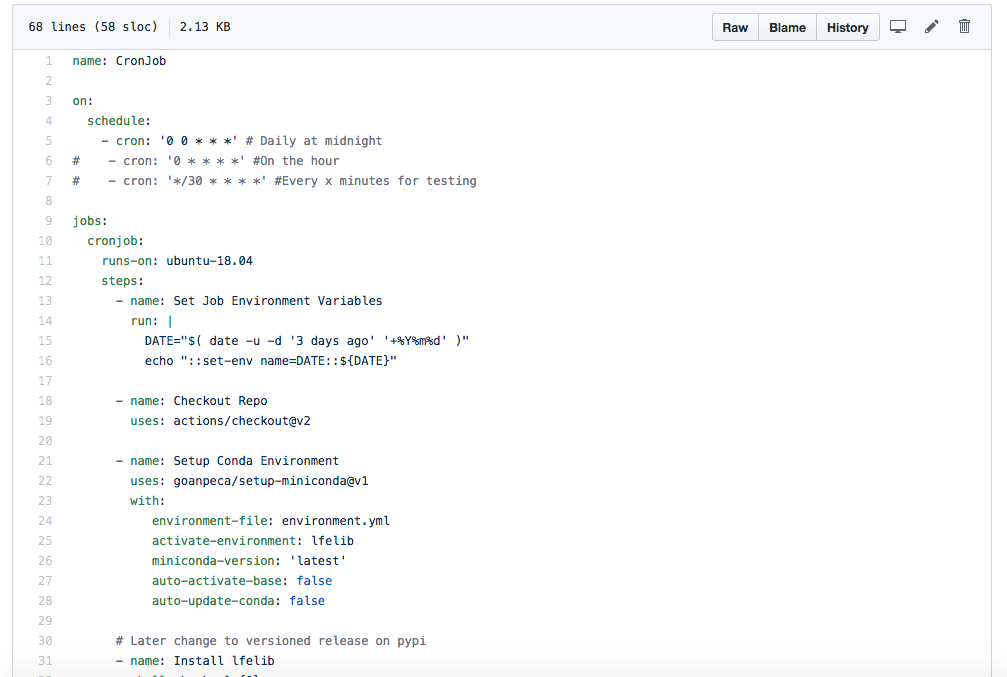
\includegraphics[width=11cm]{cronjob.png}
	\end{frame}

	\begin{frame}[fragile]
		\frametitle{Third step: GitHub workflow}
		\begin{block}{Run the job daily at midnight}
		\tiny{
		\begin{verbatim}
		  schedule:
		    - cron: '0 0 * * *' 
		\end{verbatim}
		}
		\end{block}
		\begin{block}{Get the date of three days ago}
		\tiny{
		\begin{verbatim}
		      - name: Set Job Environment Variables
		        run: |
		          DATE="$( date -u -d '3 days ago' '+%Y%m%d' )"
		          echo "::set-env name=DATE::${DATE}"
		\end{verbatim}
		}
		\end{block}
		\begin{block}{Get the conda environment to run the code}
		\tiny{
		\begin{verbatim}
		      - name: Setup Conda Environment
		        uses: goanpeca/setup-miniconda@v1
		        with:
		           environment-file: environment.yml
		           activate-environment: lfelib
		\end{verbatim}
		}
		\end{block}
		\begin{block}{Install the latest version of the package}
		\tiny{
		\begin{verbatim}
		      - name: Install lfelib
		        shell: bash -l {0}
		        run: |
		          pip install --extra-index-url https://test.pypi.org/simple/ lfelib
		\end{verbatim}
		}
		\end{block}
	\end{frame}

	\begin{frame}[fragile]
		\frametitle{Third step: GitHub workflow}
		\begin{block}{Run the script downloading the data and looking for LFEs}
		\tiny{
		\begin{verbatim}
		      - name: Run Daily Processing
		        shell: bash -l {0}
		        run: |
		          cd examples
		          ./cronscript.sh
		\end{verbatim}
		}
		\end{block}
		\begin{block}{Upload the output file}
		\tiny{
		\begin{verbatim}
		      - name: Upload Zipped LFEs Folder with Results
		        uses: actions/upload-artifact@v1
		        with:
		          name: ${{env.DATE}}
		          path: ./examples/LFEs/
		\end{verbatim}
		}
		\end{block}
		\begin{block}{Save the output file on Google Drive}
		\tiny{
		\begin{verbatim}
		      - name: Upload Results CSVs to Google Drive
		        uses: wei/rclone@v1
		        env:
		          RCLONE_CONFIG_INCUBATOR_TOKEN: ${{ secrets.RCLONE_CONFIG_INCUBATOR_TOKEN }}
		          RCLONE_CONFIG_INCUBATOR_TEAM_DRIVE: ${{secrets.RCLONE_CONFIG_INCUBATOR_TEAM_DRIVE }}
 		         RCLONE_CONFIG_INCUBATOR_TYPE: drive
		          RCLONE_CONFIG_INCUBATOR_SCOPE: drive
		        with:
		          args: copy ./examples/LFEs/ incubator:lfelib/cronjob	
		\end{verbatim}
		}
		\end{block}
	\end{frame}

	\begin{frame}
		\frametitle{Fourth step: Improving memory space and computing time}
		\begin{columns}[c]
			\begin{column}{5cm}
				\begin{block}{Memory space}
				Store instrument response into data directory
				\end{block}
			\end{column}
			\begin{column}{1cm}
				\centering
				\Huge\pointer
			\end{column}
			\begin{column}{5cm}
				\begin{block}{Memory space}
				Download instrument response before looking for LFEs
				\end{block}
			\end{column}
		\end{columns}

		\vspace{1cm}

		\begin{columns}[c]
			\begin{column}{5cm}
				\begin{block}{Computing time}
				Loop on LFE families

				\hspace{5mm} Loop on seismic stations

				\hspace{1cm} Download seismic data

				\hspace{5mm} Analyze seismic data

				\hspace{5mm} Delete seismic data
				\end{block}
			\end{column}
			\begin{column}{1cm}
				\centering
				\Huge\pointer
			\end{column}
			\begin{column}{5cm}
				\begin{block}{Computing time}
				Loop on seismic stations

				\hspace{5mm} Download seismic data

				Loop on LFE families

				\hspace{5mm} Analyze seismic data

				Delete seismic data
				\end{block}
			\end{column}
		\end{columns}
	\end{frame}

	\begin{frame}
		\frametitle{Fifth step: Saving results}
		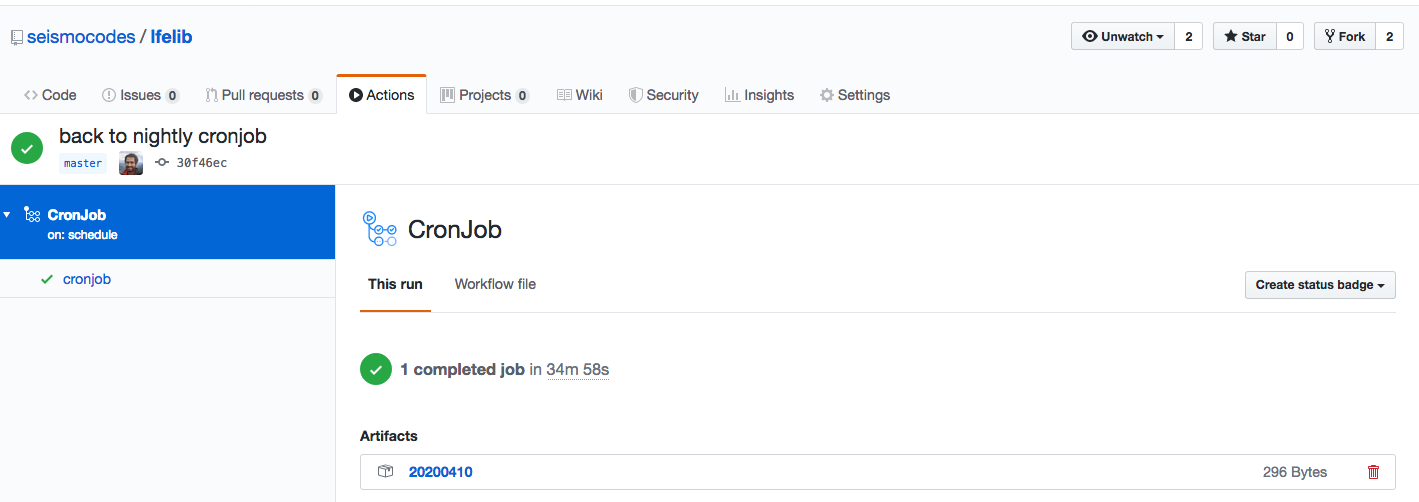
\includegraphics[width=11cm]{artifacts.png}

		\vspace{1cm}

		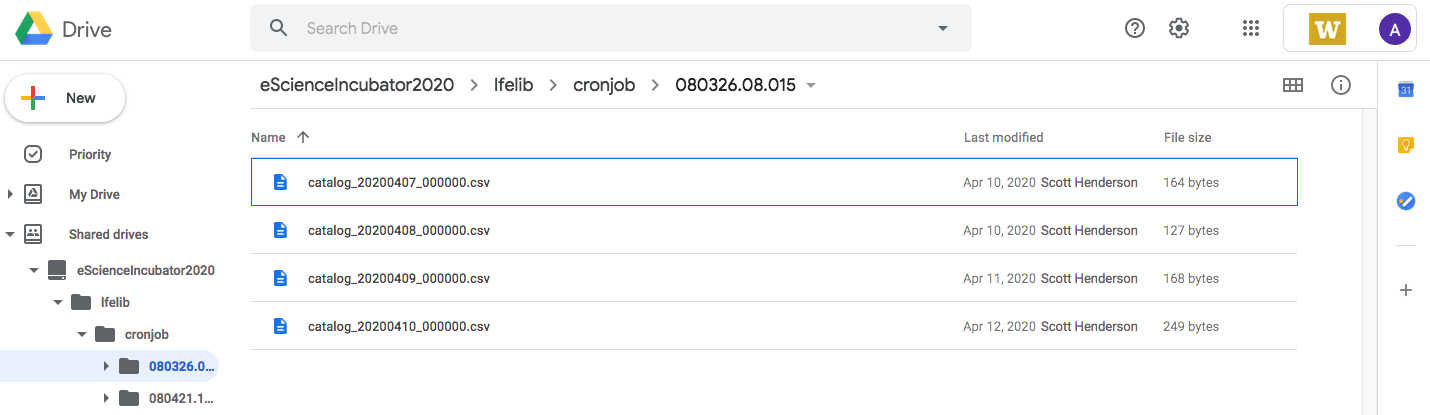
\includegraphics[width=11cm]{googledrive.png}
	\end{frame}

	\begin{frame}
		\frametitle{Future improvements}
		\begin{columns}[c]
			\begin{column}{5cm}
				\begin{block}{Computing time}
				Download data one station at a time

				Look for new LFEs one LFE family at a time
				\end{block}
			\end{column}
			\begin{column}{1cm}
				\centering
				\Huge\pointer
			\end{column}
			\begin{column}{5cm}
				\begin{block}{Computing time}
				Parallelization of Python scripts
				\end{block}
			\end{column}
		\end{columns}

		\vspace{1cm}

		\begin{columns}[c]
			\begin{column}{5cm}
				\begin{block}{Volume of data}
				Two LFE families

				Runs on GitHub in 35 minutes

				Time limit on the computing time of the jobs you can run on GitHub
				\end{block}
			\end{column}
			\begin{column}{1cm}
				\centering
				\Huge\pointer
			\end{column}
			\begin{column}{5cm}
				\begin{block}{Volume of data}
				May look at Amazon Lambda instead
				\end{block}
			\end{column}
		\end{columns}
	\end{frame}

	\begin{frame}
		\centering
		\Huge{Thank you}
	\end{frame}
\end{document}
